\documentclass{acm_proc_article-sp}
\begin{document}

\title{Gender classification using Logistic Regression}

\numberofauthors{2} %  
\author{
\alignauthor
% 1st. author
Suvir Jain,\\
\affaddr{Computer Science Department}\\
\affaddr{University of California, San Diego}\\
\email{suj011@cs.ucsd.edu}
% 2nd. author
\alignauthor
Gaurav Saxena\\
\affaddr{Computer Science Department}\\
\affaddr{University of California, San Diego}\\
\email{gsaxena@cs.ucsd.edu}
}

\maketitle
\begin{abstract}
Gender classification is important in several applications like tailoring personalized experience of stores and gadgets, providing analytics data to companies about customers etc. We use 800 different features to train a Logisitc Regression model to achieve this task. We report the performance of Logistic Regression using Stochastic Gradient Descent and L-BFGS. Furthermore, to protect model from over-fitting, we use cross validation and $L_{2}$ Regularization. In our experiments with test data we found that our model was able to identify the correct labels 92\% of the time
\end{abstract}

\section{Introduction}
$R4 \⋈_C3 R3 \⋈_C2 R2 \⋈_C1 R1$
Logistic Regression is a statistical classification model to determine the probabilities of the outcomes based on the occurrence of certain features. The process of deriving this model is called training the model. This process finds weights for the features such that their linear combination can be used to determine the 'most probable' outcome. However, linear models are unbounded and thus, they cannot be directly used to calculate the probabilities, which are bounded between 0 and 1. To achieve these bounds this process uses a squashing function which reduces the range of the linear function to be between 0 and 1.

To train this model a data set is used, which contains various observations of an experiment. Each observation of the experiment consists of the features and the outcome. For example, let us consider an observation of the the data set [1] for gender classification. Each observation of this data set consists of 800 features and their values for a person. It also contains a label to identify the person as male or female. This label acts as the outcome of the experiment.

This data can be used to deduce the optimal values of the weights for the features by solving a system of non-linear equations in 800 variables. However, achieving this by mathematical methods may be intractable. Thus, numerical methods like Gradient Descent[2] are used to find optimal values. \\
However, gradient descent for large data sets tend to be slow. This is because it has a time complexity of $O(n^{2}d)$[3] where n is the number of observations and d is the number of dimensions. Thus, we use other numerical methods like Stochastic Gradient Descent(SGD) and L-BFGS which are less accurate but are faster [4].

Although, numerical methods make hard mathematical problems tractable, their convergence is dependent on a number of parameters. These parameters are called hyperparameters. Better hyperparameters can result in better results(global optima), faster convergence and less over-fitting (by using regularization). Unfortunately, trial and error is the only way to determine the them. Determination of hyper parameter by trial and error is called grid search[4]. To reduce the time taken to determine the best hyperparameters, we increase them in geometric progression.

We make four major contributions. First, we use the data set in the running example to train a model using logistic regression using SGD and L-BFGS. We do experiments to compare the running time of Gradient Descent, SGD and L-BFGS. Secondly, we have used regularization and cross-validation to prevent the model over-fitting the data. We report the performance of the model with and without these measures. Thirdly, we also report the accuracy of the model on cross-validation and test data set. Finally, we discuss our results, the strengths and weaknesses of our approach.

\section{Preliminaries}
Let us formalize the arguments presented above. We use a scheme similar to the one discussed in [5]. For the rest of the report we assume that capital letters like $Y, X$ refer to a variable and small letters like $y, x$ refers to their values. We also assume that the outcome of the experiment, $Y$ is dichotomous and can have values ${0,1}$ only, while $X$ can have any real value. Now, let us consider an observation $j$ of the experiment. The outcome of this experiment is denoted by $Y$ and can take any of the two values ${0,1}$. Outcome of an observation $j$ is denoted by $y_{j}$. The features, in the observation $j$, are denoted by a vector $x_{j}=(x_{1}, x_{2},...x_{d})$ where d is the number of dimensions. 
\subsection{Logistic Regression}
We use the principle of conditional likelihood\cite{efron1975efficiency} to calculate $\beta_{1},\beta_{2},...\beta_{m}$ such that the probability 

$P(Y|X) = \prod\limits_{1}^n (p_{i})^{y_{i}}(1-p_{i})^{(1-y_{i})}$ is maximum. In logistical regression, the probability $p_{i}$ takes the following form
\begin{align}
P(y|x)=\dfrac{1}{1+e^{-(\beta_{0}+\sum\limits_{j=1}^n \beta_{j}x_{j})}}
\end{align}
where $\sigma=\dfrac{1}{1+e^{z}}$ is the squashing function\\
and $\beta_i$ is a weight associated with $x_i$

It is hard to do numerical calculations with conditional likelihood because computers run into underflows. Therefore, we maximize the log-likelihood $log(P(y|x)$, instead of the likelihood function. This is called log conditional likelihood(LCL). Therefore, first partial derivative of log-likelihood takes the following form

\begin{align}\label{eq:max}
\dfrac{\partial(log(P(y|x))}{\partial\beta_{j}} = \sum\limits_{i=1}^n(y_i-p_i)x_{ij}
\end{align}

\subsection{Gradient Descent}
We solve equation \ref{eq:max} using gradient descent[6], which takes the following form

\begin{align}\label{eq:betaUpdate}
\beta_j \gets \beta_j + \lambda\sum\limits_{i=1}^n(y_i-p_i)x_{ij}
\end{align}
where $\lambda$ is called learning rate and is independent of the observations

Gradient descent can only be used to maximize a convex function because it converges to the local optima. Since a convex function has only one optima, gradient descent can be used to maximize it. A function is a convex function if its second derivative is always positive. As the equation below shows, log likelihood is a convex function

\begin{align}
\dfrac{\partial^2(log(P(y|x))}{\partial\beta_{j}^2} = -\sum\limits_{i=1}^np_i(y_i-p_i)x_{ij}^2
\end{align}

The equation \ref{eq:betaUpdate} implies that for each $\beta_j$ update, sum over all the observations is required. In practise, this turns out to be slow. Therefore several other methods have been developed to improve the performance of the convergence algorithm. We discuss two such methods used in our experiments,1) SGD 2)L-BFGS.
\\
\subsubsection*{Stochastic Gradient Descent}
SGD proposes that instead of calculating each $\beta_j$ over all the observations, the process can be randomized. Thus, for an observation $i$ the update rule \\ref{eq:betaUpdate} can update all $\beta_j$ once. Due to its random nature, this process is called stochastic gradient descent.
\subsubsection*{Limited Memory Broyden-Fletcher-Goldfarb-Shanno algorithm (L-BFGS}
L-BFGS is a quasi-Newton optimization method which approximates the Hessian matrix to optimize likelihood. We do not go into the details of the algorithm here and readers are encouraged to read \cite{malouf2002comparison}
\subsection{Feature Scaling}
Feature scaling is used standardize the vectors of the observations of an experiment. Feature scaling is generally done to ensure that widely varying vectors can be evaluated at the same scale\cite{bro2003centering}. It also helps in computation as large values of features can cause overflows, without affecting the fit of the data. We scale the input vectors by their Euclidean norm.
\subsection{Over-Fitting}
Overfitting is defined as a characteristic of a regression model which is based on the bias of the sample at hand\cite{babyak2004you}. Overfitting leads to optimistic models which perform well on a training set but fail to produce similar results on a validation set. We discuss two, among many, ways to reduce overfitting, which we have used in our experiments
\subsubsection*{Validation}
The process of validation includes dividing the training set into two parts namely, the training set and the validation set. The training set is used to train the model and the validation set is used to determine the goodness of the fit. A good fit is determined when accuracy of validation set diverges as compared to the training set. The ratio of the number of examples in the validation set is determined by taking into account the number of training set examples which may represent the model adequately and therefore is not standard. Therefore we split the 70\% input data set as training set and the rest as validation set.
\subsubsection*{Regularization}
Regularization is the process of encouraging the parameters to be small especially when the number of observations are smaller than the number of dimensions\cite{ng2004feature}. We use $L_2$ Regularization which subtracts the sum of parameters from the log likelihood. It has a property that it reduces over-fitting as it penalizes the model for large parameter values due to its square term.

\section{Implementation}
Mention that we are not using centering using mean because it is only useful when the a dimension is offset by a constant factor\cite{bro2003centering}. For example, if height is a dimension then, it can be expected that most dimension values will be more than 1m. Since we do not know for sure if that is the case with our data, we do not use centering.
http://www.willamette.edu/~gorr/classes/cs449/overfitting.html
Describe randomization
\subsection{SGD}
\subsubsection{Normalization of training data}
We found that the feature values in the training data varied quite a lot. Many rows had a difference of more than 100 between the maximum and minimum feature values. This would have skewed the results in favor of features with larger magnitudes. We normalized the feature vectors by dividing each feature value by the norm of the entire row's feature vector. This helped scale all feature values to a range between +1 and -1. It also preserved the relative ratios between the values of different features. 
\subsubsection*{Tuning the learning rate}
Tuning the learning rate $\lambda$ turned out to be a non-trivial challenge. We found that using a single value of learning rate caused logistic regression to converge fast for some values of hyperparameter $\mu$ and very slowly for other values. 
\paragraph{Method 1}
Having realized that we need a more sophisticated approach, we started with reducing the learning rate as the $\bigtriangledown(LCL)$ approached zero. Initially, we simply divided the learning rate by 5 when the $\bigtriangledown(LCL)$ reduced to a value less than a certain threshold. This threshold was set at 1. We also divided the threshold by 5 every time that it was breached. This meant that the learning rate was updated whenever $\bigtriangledown(LCL)$ breached 1,0.2,0.04. Previous to using this method, the $\bigtriangledown(LCL)$ used to overshoot the convergence value. After using this method, the algorithms converged in less than 100 iterations.
\paragraph{Method 2}
We used a method described in \cite{settingHyperparameters}. Learning rate was updated according to the formula $\lambda_0/(1+\lambda_0*c*e)$. Based on a few experiments, we set the value to L0 to 0.02 and the value of c to 1.5. \textit{e} was the number of epochs that had elapsed. This method resulted in faster convergence than the method described above.

\subsection{Tuning the initial guess}
We thought that the best initial guess for the parameters of the model will be the one which takes the conditional likelihood(CL) to its highest value. We approximated the CL function for linear regression to the one below, assuming all $\beta$ to be equal

\begin{align}
\dfrac{e^{k * \beta}}{1 + e^{n * \beta}}
\end{align}
where k is the number of observations with y = 0\\
and n is the number of observations


We used wolfram aplha\cite{} to plot this and find an x which leads to a the maximum CL. Similarly, we used the following function to find the initial guess of regularized model

\begin{align}
\dfrac{e^{k * \beta}}{1 + e^{n * \beta}} - \mu||\beta||^2
\end{align}
where k is the number of observations with y = 0\\
and n is the number of observations

\subsection{L-BFGS}
For L-BFGS, we used the \textsc{matlab} implementation referenced in the project description \cite{lbfgsMatlabImpl}.

\section{Experiments}
In our study of classifying observations into gender classes using logisitc regression, we used two algorithms namely SGD and L-BFGS.

\begin{figure}\label{SGD_(not_Regularized)_Accuracy_vs_Epochs}
\centering
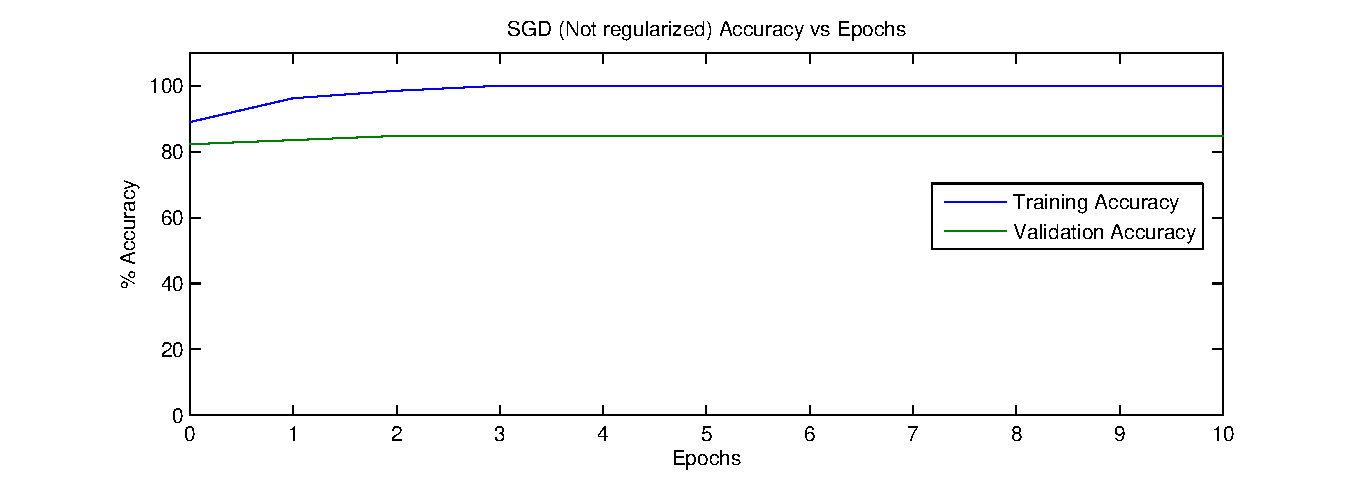
\includegraphics[scale=0.4]{SGD_(not_Regularized)_Accuracy_vs_Epochs.eps}
\caption{Stochastic Gradient Descent: Accuracy of trained models improves with number of training epochs}
\end{figure}

\begin{figure}\label{accuracy_vs_epochs_l2_regularized}
\centering
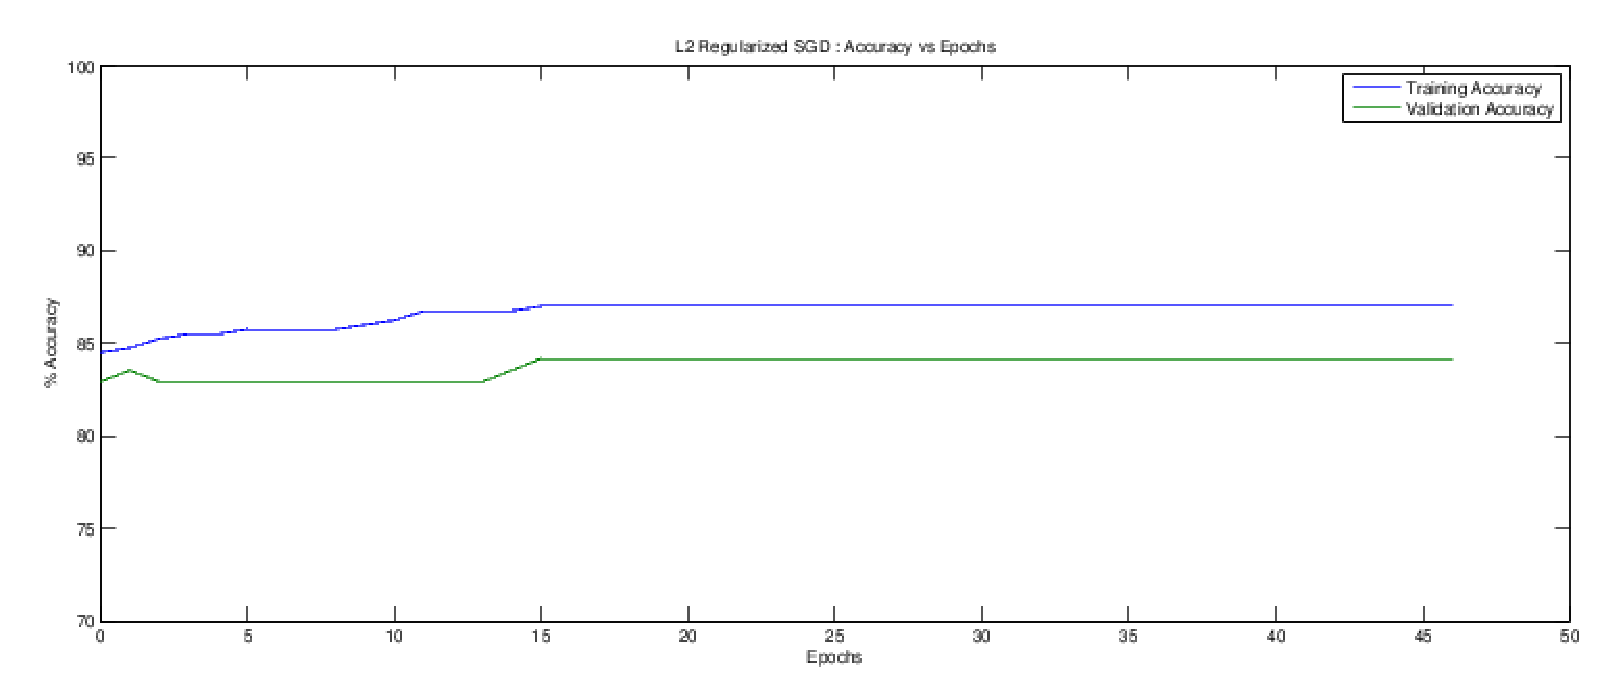
\includegraphics[scale=0.25]{accuracy_vs_epochs_l2_regularized.eps}
\caption{$L_{2}$ Regularized Stochastic Gradient Descent : Accuracy of trained models improves with number of training epochs}
\end{figure}

\begin{figure}\label{SGD_Regularized_Log_Likelihood}
\centering
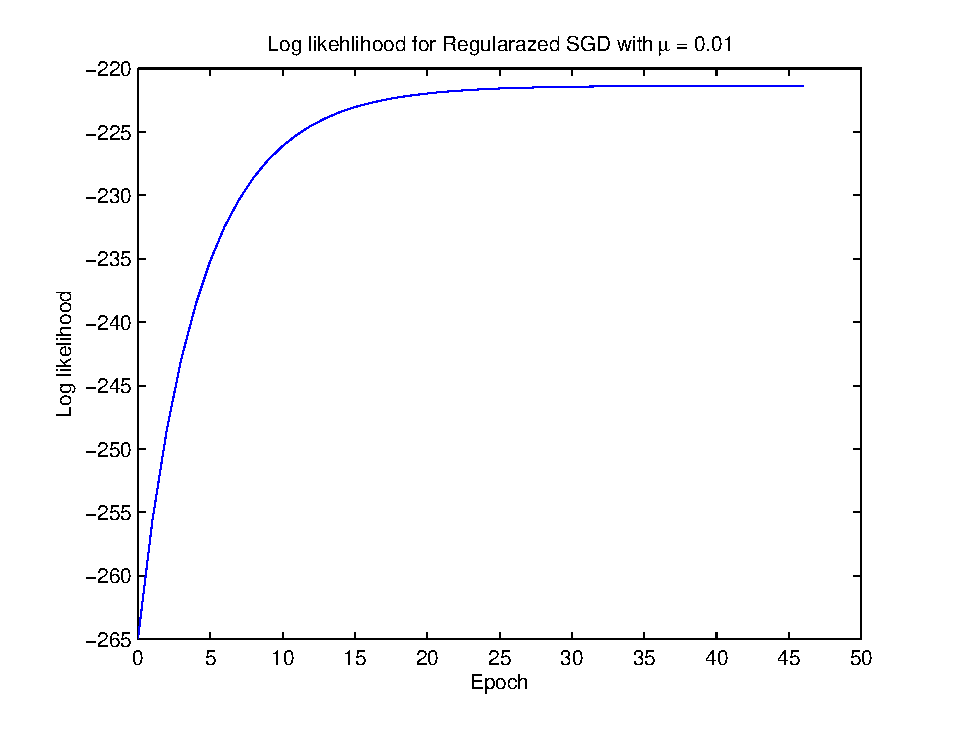
\includegraphics[scale=0.5]{Regularized_Log_Likelihood.eps}
\caption{$L_{2}$ Regularized Stochastic Gradient Descent :Regularized LCL vs Number of Epochs}
\end{figure}

\begin{figure}
\centering
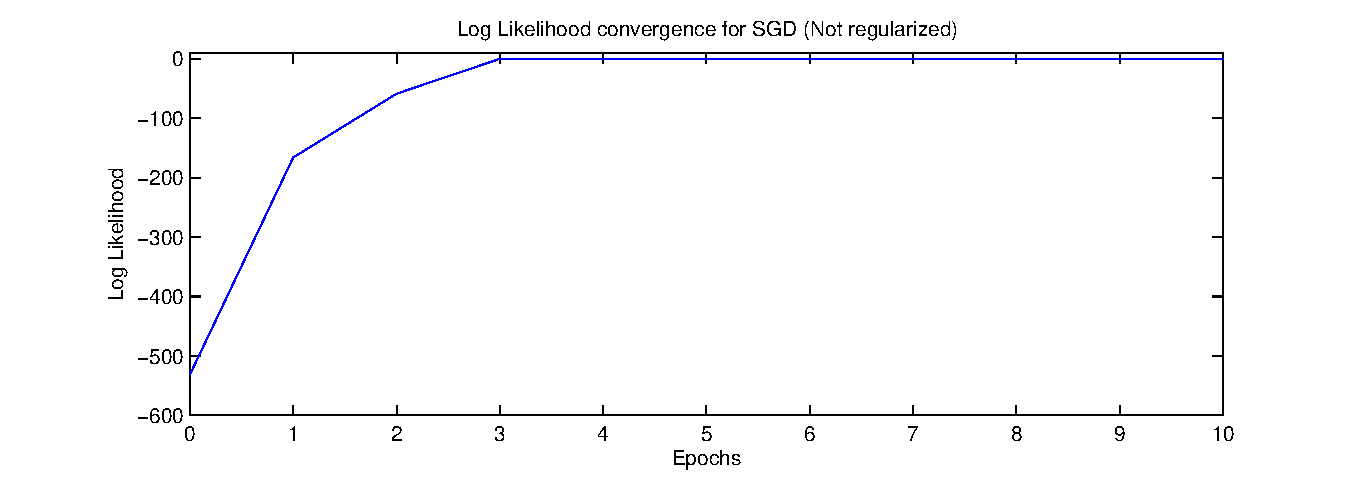
\includegraphics[scale=0.4]{Log_likelihood_for_SGD_(Not_Regularized).eps}
\caption{Stochastic Gradient Descent : LCL vs Number of Epochs}
\end{figure}

SGD implementation was done both with and without regularization until convergence as shown in \ref{SGD_Regularized_Log_Likelihood} and \ref{SGD_(not_Regularized)_Accuracy_vs_Epochs} the process converged to a stable value As shown in \ref{SGD_(not_Regularized)_Accuracy_vs_Epochs} SGD and \ref{accuracy_vs_epochs_l2_regularized} without regularization seems to converge faster. This could be attributed to the fact that inverse dampening worked when used with SGD without regularization but did not when it was used with SGD with regularization. This is because the learning rate becomes smaller faster than SGD could converge. Any change in SGD beyond that point was very small and we realized that using inverse dampening could be counter-productive when used with regularization. Thus, we used constant learning rate for SGD with regularization. We believe that more experiments with more diverse data sets need to be performed to say if this process works better.

In both these experiments, we measured validation accuracy with test accuracy. We hypothesize that as model reaches convergence, it validation accuracy increases and it tops when model is just right. As model is tried to be fit on further epochs, it overfits the training data. Hence, may not represent the best model. Accordingly, we found that validation accuracy first increases with epochs and after achieving the maximum, it decreases before becoming constant. We take models of the parameters at the point validation accuracy is maximum, instead of the point where validation accuracy stabilizes. This process did improve the accuracy of the model on test marginally, but, we did not find a sizeable difference in the performance of model.

\begin{figure}\label{accuracy_vs_mu_l2_regularized}
\centering
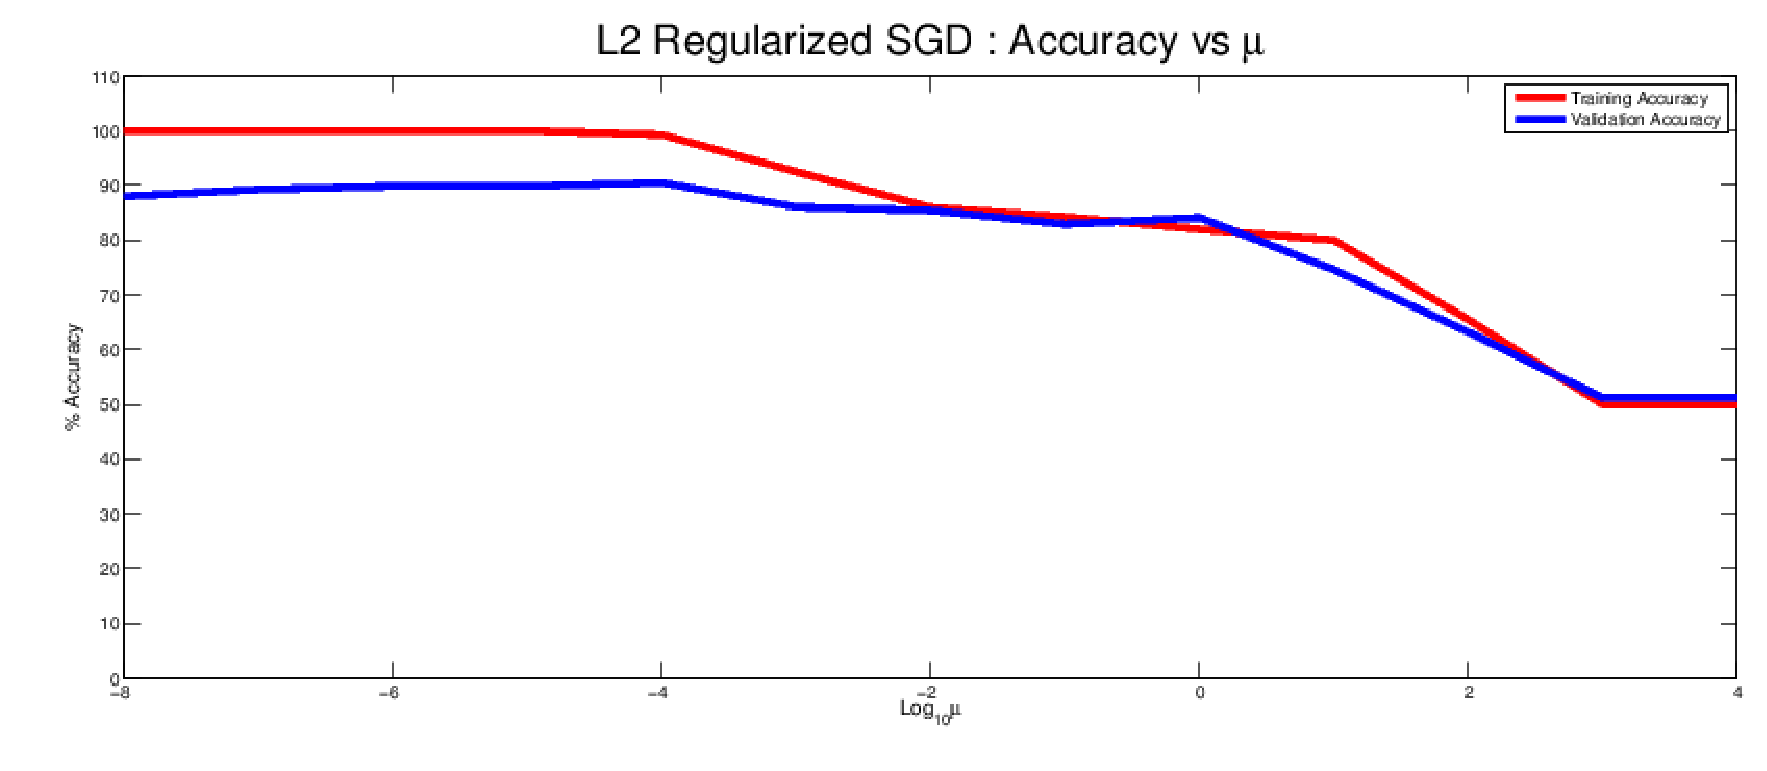
\includegraphics[scale=0.25]{accuracy_vs_mu_l2_regularized.eps}
\caption{$L_{2}$ Regularized Stochastic Gradient Descent : Accuracy vs Hyperparameter $\mu$}
\end{figure}

Derivation of the model with regularization also requires grid search for a hyperparameter called strength of regularization $\mu$. As shown in figure \ref{accuracy_vs_mu_l2_regularized} we find the value of $\mu=10^{-2}$ where validation accuracy is equal to the training accuracy. We think that this is a good trade-off between over-fitting and model accuracy.

During the grid search, for different $\mu$ we used different learning rates, $\lambda$ for faster convergence. We noticed that smaller $mu$ required smaller $\lambda$. We did not investigate a precise relationship between these parameters since learning rate only helps in faster convergence and doesn't contribute to accuracy of the model. As shown in figure \ref{accuracy_vs_mu_l2_regularized}, as $\mu$ decreases, the accuracy of the model increases. We expected accuracy to decrease with $\mu$ but we did not observe that trend. We think that this is because feature set is comprehensive enough to represent the model and therefore regularization doesn't vastly improve peak performance. Therefore, we find that for lower values of regularization, the accuracy tends to the unregularized SGD model.

\subsection{L-BFGS}
\begin{figure}\label{LBFGS_Graph}
\centering
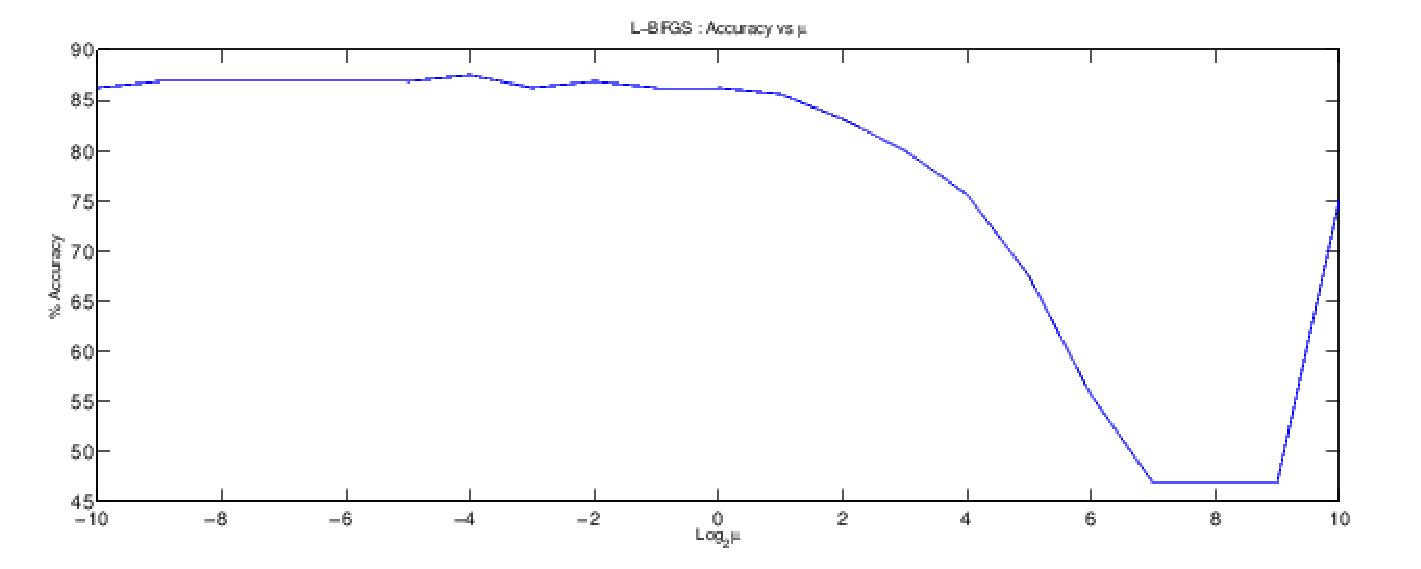
\includegraphics[scale=0.4]{LBFGS_Graph.eps}
\caption{L-BFGS : Accuracy vs parameter $log_2{\mu}$}
\end{figure}

The only tunable parameter in this implementation is vector of values that has to be input to the algorithm. This parameter was varied in steps from $2^{-10}$,$2^{-9}$,$2^{-8}$ ... $2^{9}$,$2^{10}$. The optimum weight vector for each of these parameters was recorded. The optimal model was achieved for parameter value $2^{-6}$. We then calculated the accuracy of this model using the validation set. The model which fit the validation set with the highest accuracy was used to predict values on the test set. Refer to figure \ref{LBFGS_Graph}.

\begin{figure}\label{All_accuracies_in_one}
\centering
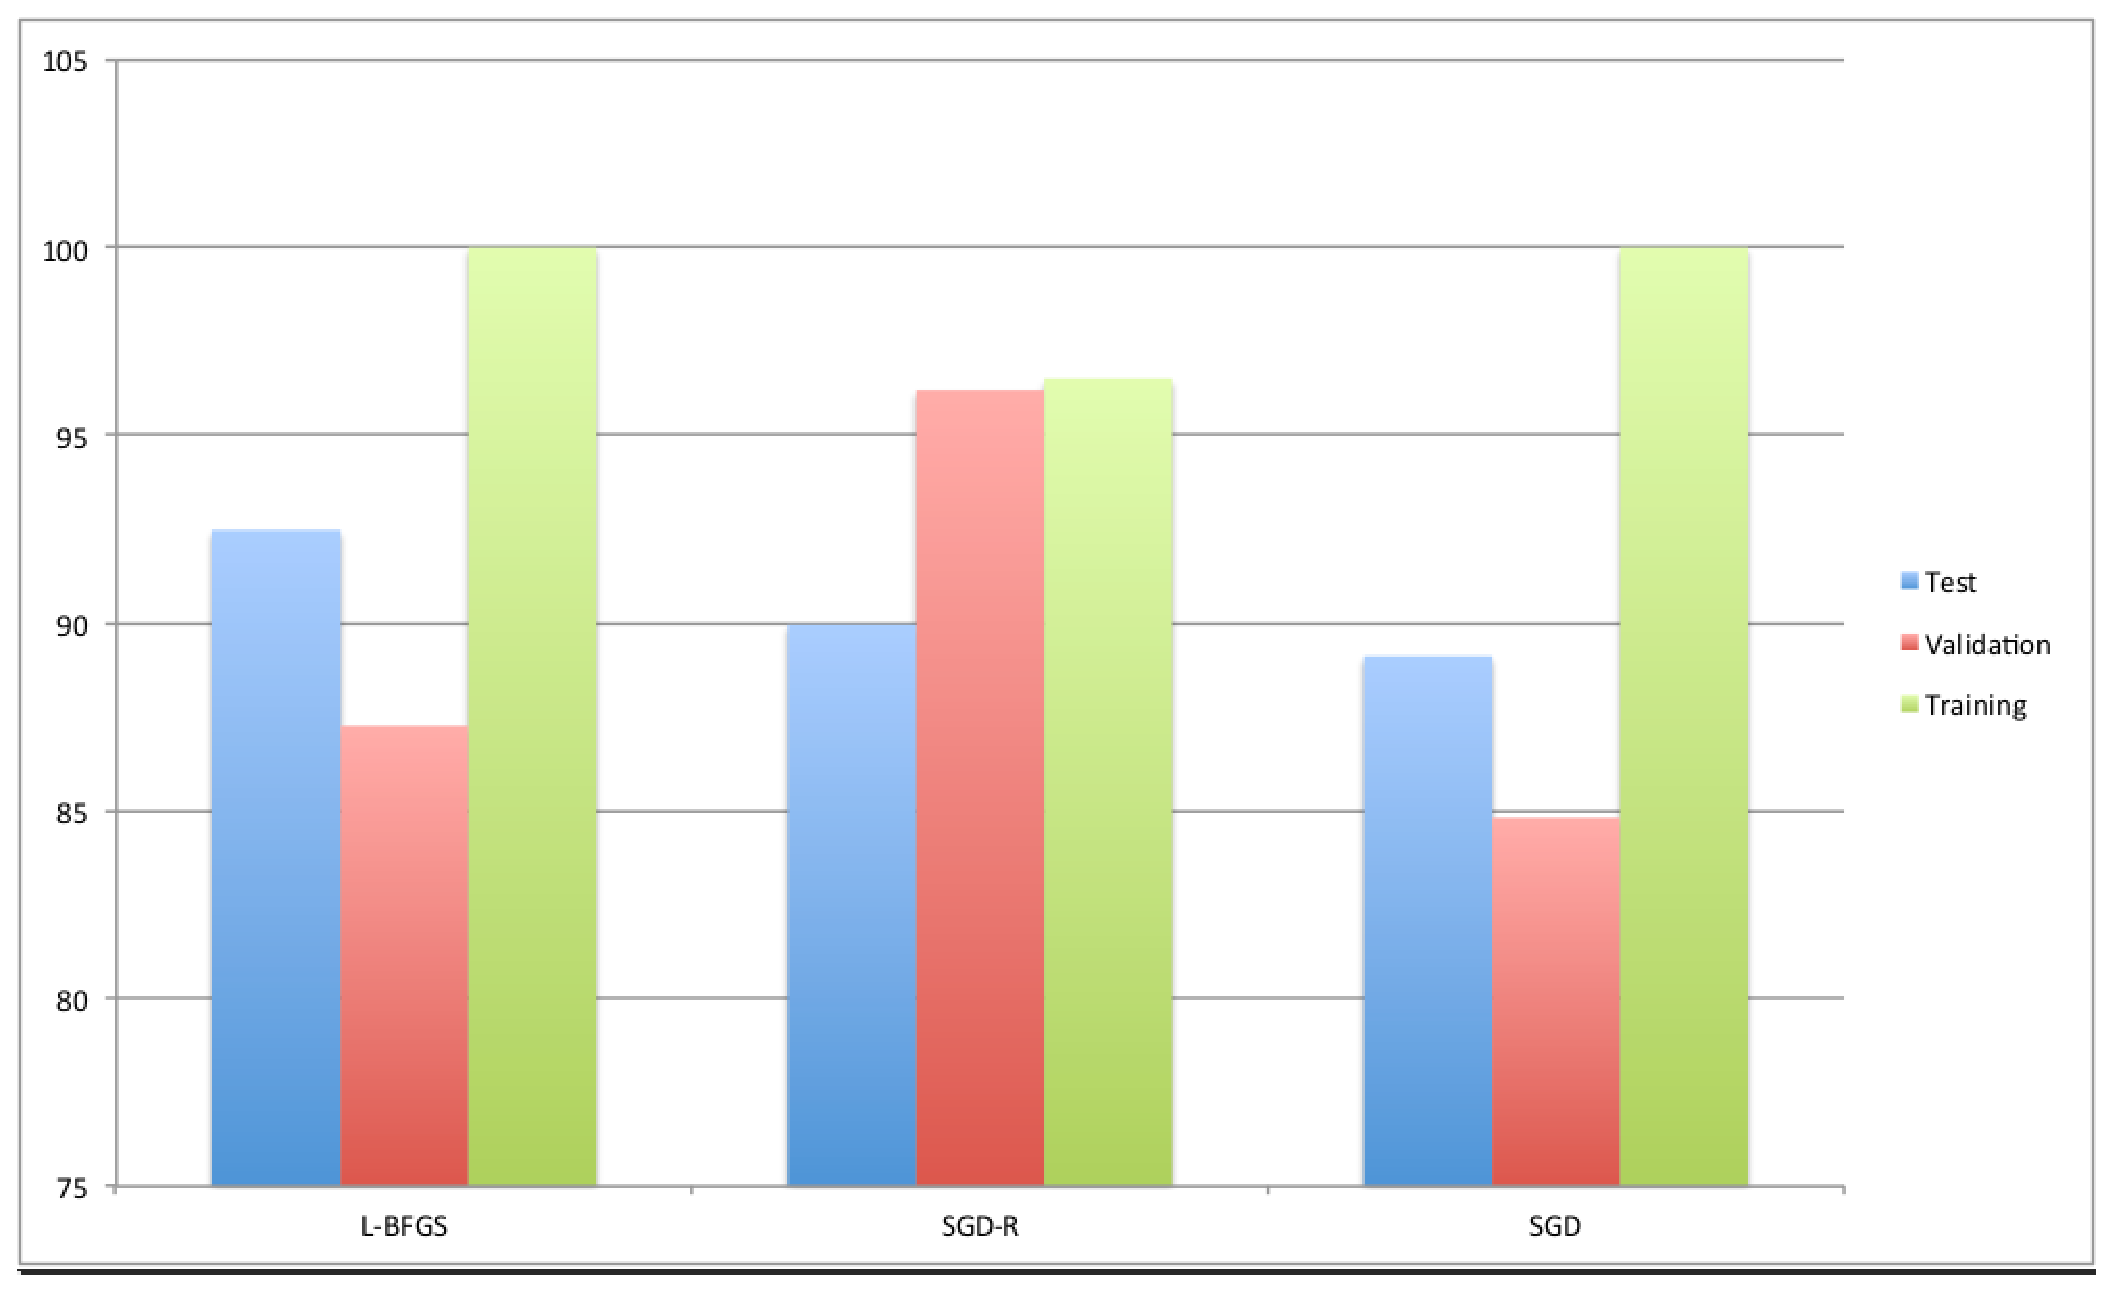
\includegraphics[scale=0.25]{All_accuracies_in_one.eps}
\caption{Accuracies for all SGD variants - $L_{2}$ Regularized and vanilla SGD}
\end{figure}
\bigskip
\subsection{Accuracy}
The model we derive seems to be a good fit to the data as we get comparable accuracy as other implementations \cite{mpComp}. As shown in figure \ref{All_accuracies_in_one} we consistently achieve about 90\% accuracy when model is run on test set for all our experiments namely SGD without regularization, SGD with regularization and L-BFGS. Our model also shows similar accuracy on validation set, which shows that we could avoid overfitting of the model on training set; though, accuracy of model on training set does reach 100\% in case of SGD without regularization and L-BFGS. We also notice that  adding regularization reduces overfitting as training data doesn't reach 100\% accuracy for SGD with regularization while the model still maintains a good accuracy on test and validation set.

\section{Conclusion}
We have presented a nuanced analysis of two major optimization algorithms used in logistic regression  - Stochastic Gradient Descent and L-BFGS. Using grid search, we learned the optimal value of the hyperparameter. Tuning the learning rate turned out to be one of the most difficulat parts of using SGD.\\
Due to the small size of training set, overfitting was always a challenge. However, using $L_{2}$ regularization helped reduce any overfitting to a great extent. The reported accuracy values(\ref{All_accuracies_in_one}) show an acceptable error rate (about 10\%) for both regularized models.
\\
One of the drawbacks of this model is that it has been trained on a data set where the number of training examples is far fewer than the number of features. Better models could have been developed with more data.
1. Comparison of number of iterations, accuracy on training set, accuracy on validation set, accuracy on test set for GD vs SGD vs LGBFS\\
Discussion
2. Comparison of accuracy of training set, validation set, test set for no regularization, regularization, and regularization without intercept\\
%
% The following two commands are all you need in the
% initial runs of your .tex file to
% produce the bibliography for the citations in your paper.
\bibliographystyle{abbrv}
\bibliography{Report} 
\end{document}
